\documentclass[letterpaper,12pt]{article}
\usepackage[margin=14mm,top=18mm,bottom=17mm,headheight=14pt]{geometry}
\pdfmapfile{+cm.map}\pdfmapfile{+cmextra.map}
\usepackage{tikz,fancyhdr,amsmath,amssymb}
\usetikzlibrary{arrows.meta,patterns}
\pagestyle{fancy}\fancyhf{}\renewcommand{\headrulewidth}{0pt}
\fancyhead[L]{\small Week 48 / Inside and outside covers / K--1}
\fancyfoot[L]{\small Bellingham Math Circle / Week 48 / F48-K-v2}
\fancyfoot[R]{\small\thepage}
\setlength{\parindent}{0pt}\setlength{\parskip}{0pt}
\begin{document}
\noindent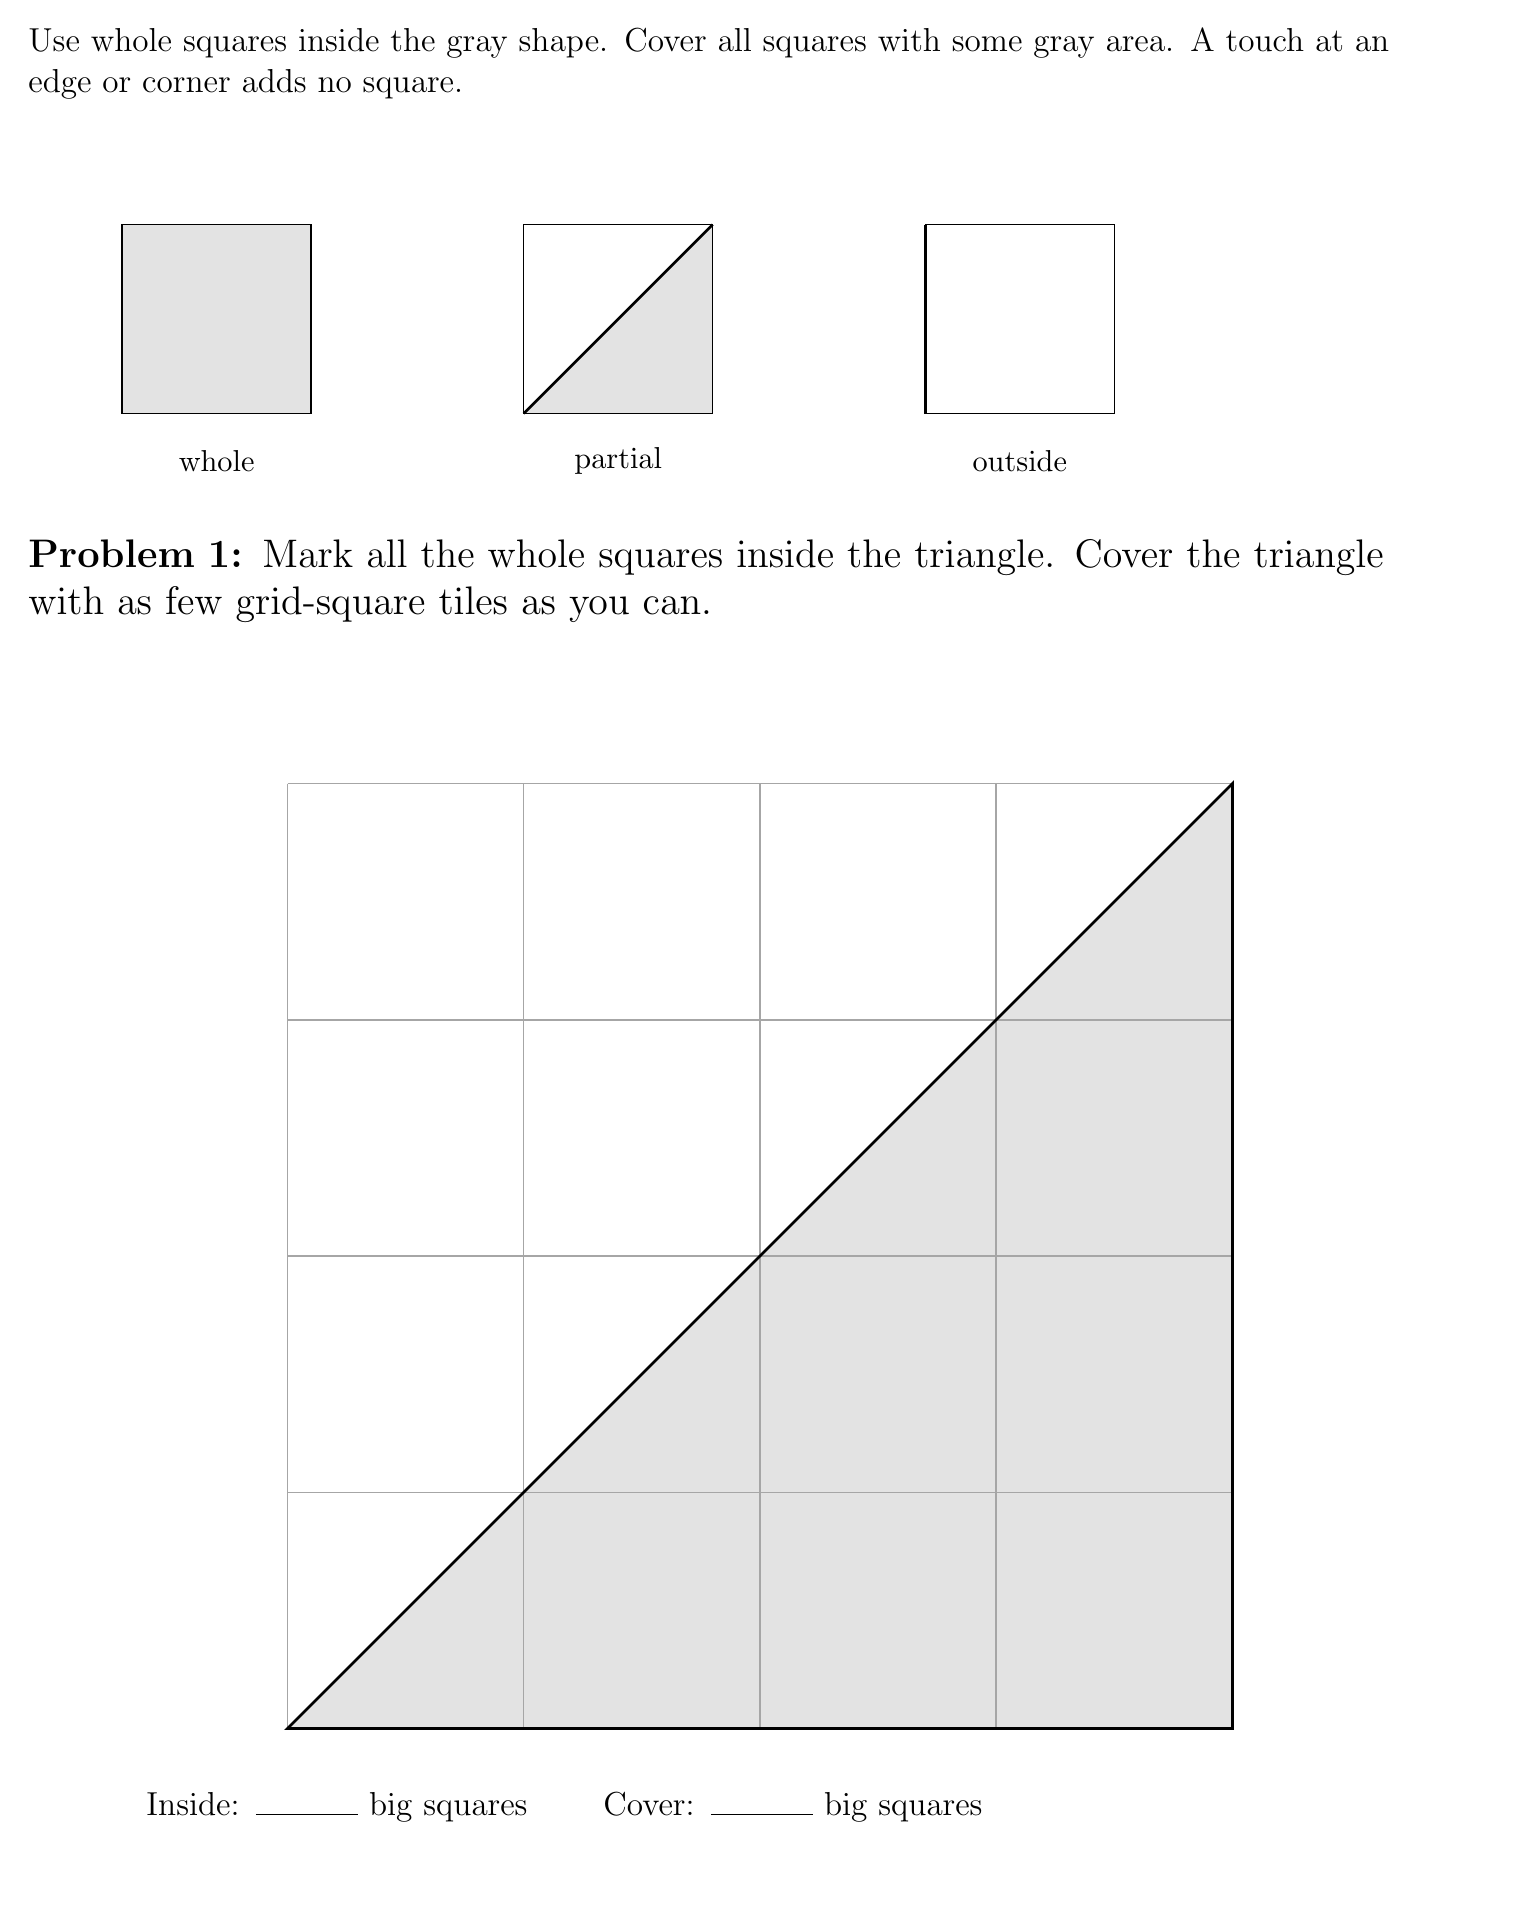
\begin{tikzpicture}[x=1mm,y=-1mm,line width=.5pt]
\path[use as bounding box] (0,0) rectangle (185,235);
\node[anchor=north west,inner sep=0pt,text width=180mm,font=\fontsize{12}{15}\selectfont] at (0,0) {Use whole squares inside the gray shape. Cover all squares with some gray area. A touch at an edge or corner adds no square.};
\draw[fill=gray!22] (12,25) rectangle ++(24,24);
\node[anchor=center,inner sep=1pt,font=\fontsize{11}{13}\selectfont] at (24,55) {whole};
\fill[gray!22] (63,49)--(87,49)--(87,25)--cycle;
\draw[] (63,25) rectangle ++(24,24);
\draw[line width=1pt] (63,49) -- (87,25);
\node[anchor=center,inner sep=1pt,font=\fontsize{11}{13}\selectfont] at (75,55) {partial};
\draw[] (114,25) rectangle ++(24,24);
\draw[line width=1.2pt] (114,25) -- (114,49);
\node[anchor=center,inner sep=1pt,font=\fontsize{11}{13}\selectfont] at (126,55) {outside};
\node[anchor=north west,inner sep=0pt,text width=180mm,font=\fontsize{14}{17}\selectfont] at (0,65) {\textbf{Problem 1:} Mark all the whole squares inside the triangle. Cover the triangle with as few grid-square tiles as you can.};
\fill[gray!22] (33.0,216.0) -- (153.0,216.0) -- (153.0,96.0) -- cycle;
\draw[gray!70] (33.0,96) -- (33.0,216);
\draw[gray!70] (33,96.0) -- (153,96.0);
\draw[gray!70] (63.0,96) -- (63.0,216);
\draw[gray!70] (33,126.0) -- (153,126.0);
\draw[gray!70] (93.0,96) -- (93.0,216);
\draw[gray!70] (33,156.0) -- (153,156.0);
\draw[gray!70] (123.0,96) -- (123.0,216);
\draw[gray!70] (33,186.0) -- (153,186.0);
\draw[gray!70] (153.0,96) -- (153.0,216);
\draw[gray!70] (33,216.0) -- (153,216.0);
\draw[line width=1pt] (33.0,216.0) -- (153.0,216.0) -- (153.0,96.0) -- cycle;
\node[anchor=north west,inner sep=0pt,text width=180mm,font=\fontsize{12}{15}\selectfont] at (15,224) {Inside: \rule{13mm}{.3pt} big squares \qquad Cover: \rule{13mm}{.3pt} big squares};
\end{tikzpicture}
\newpage
\noindent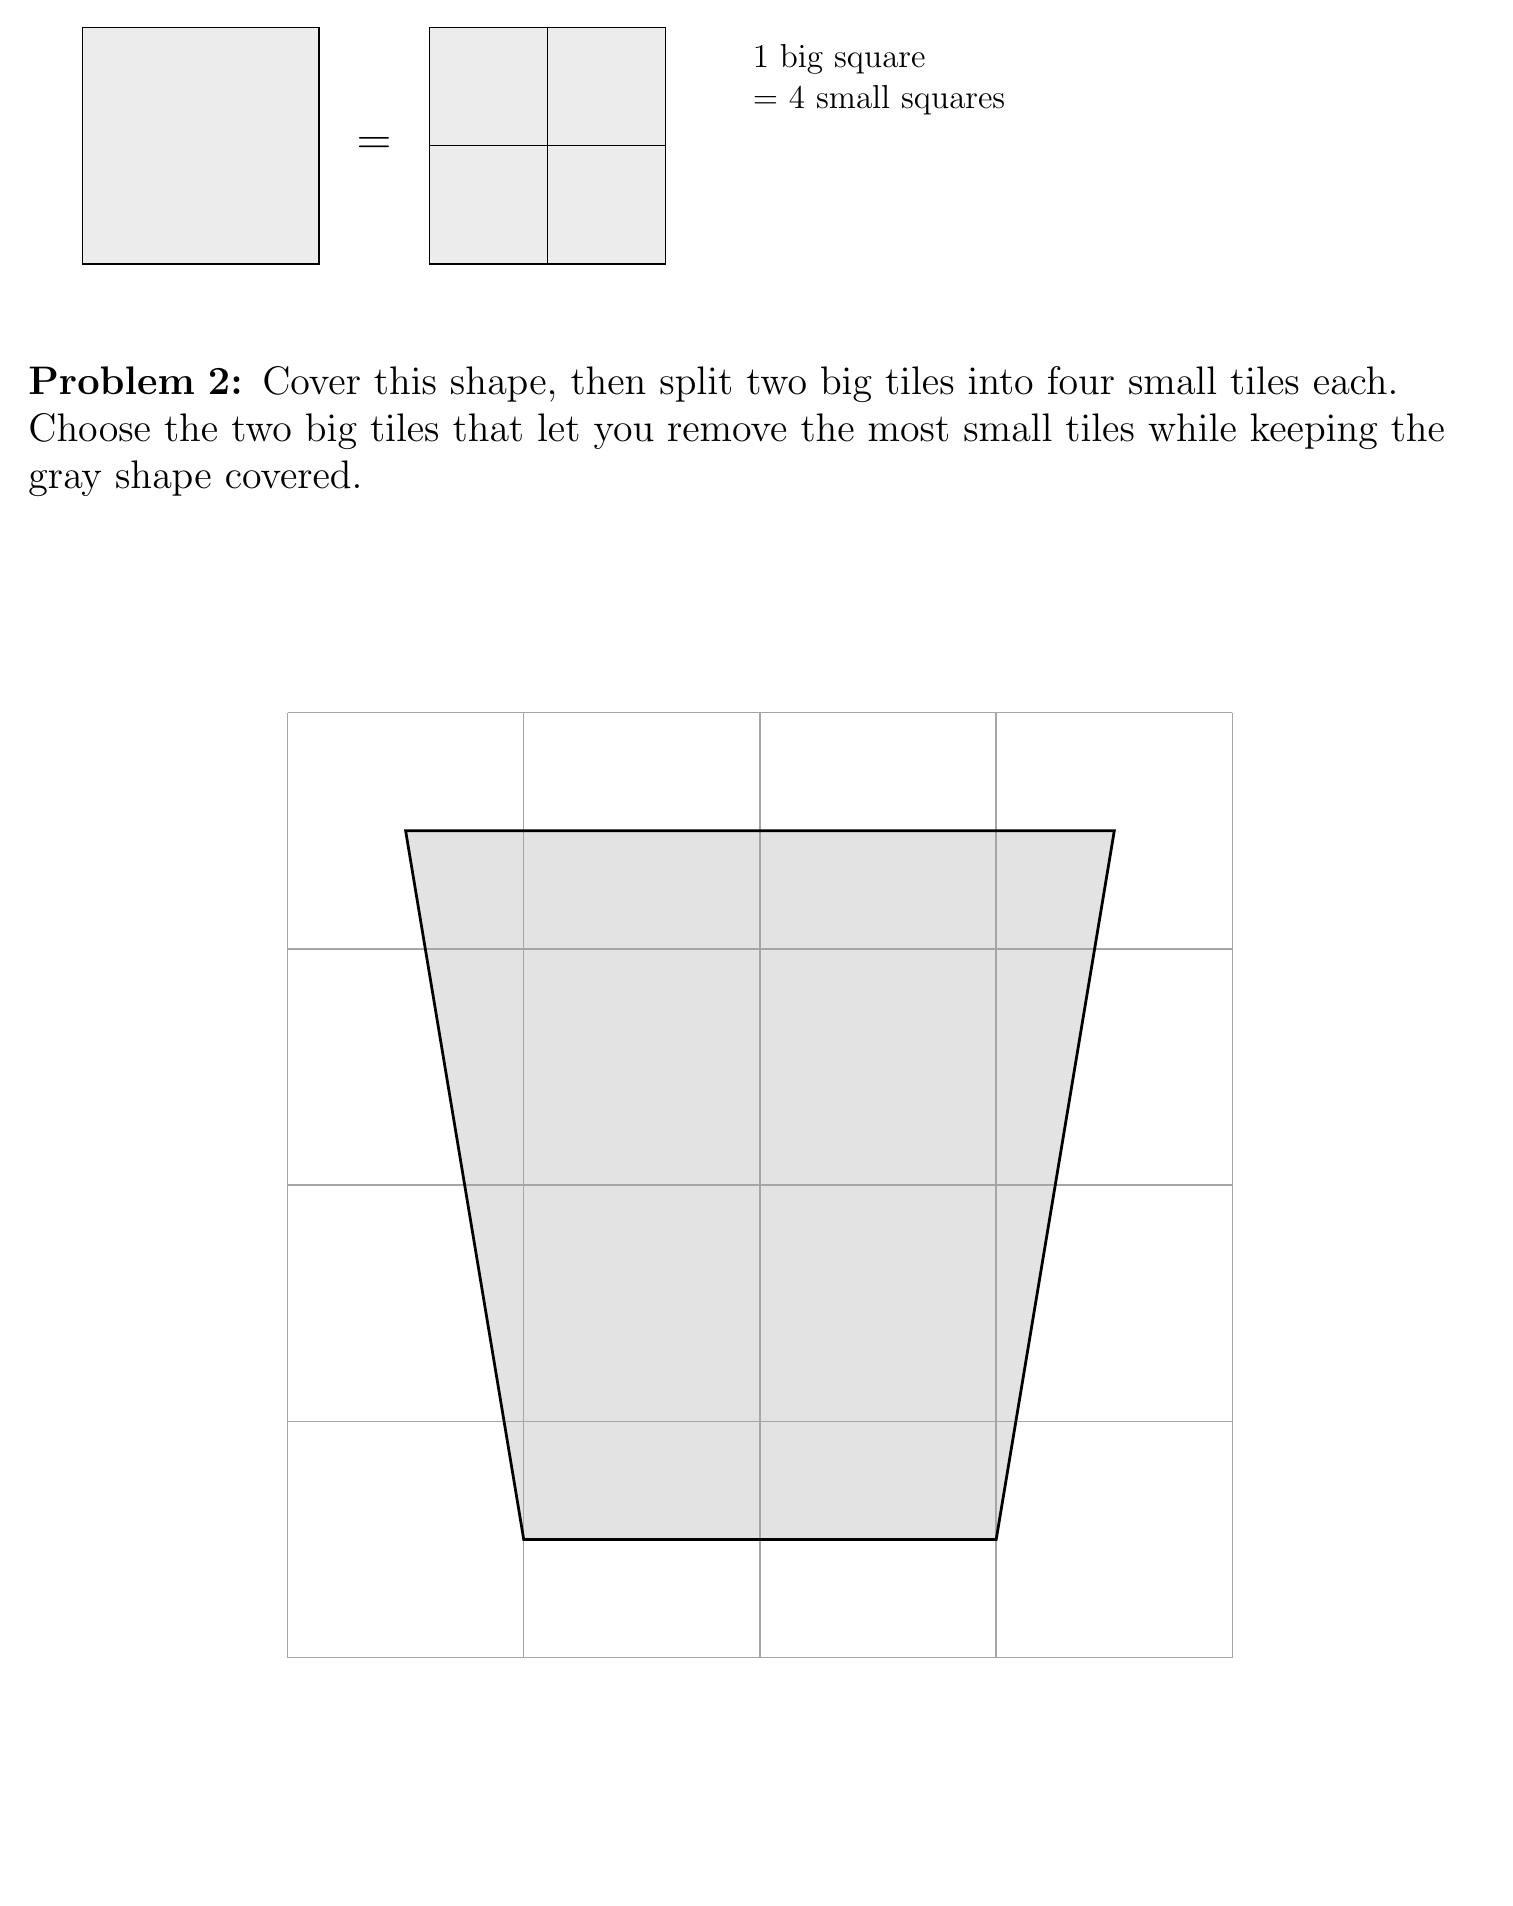
\begin{tikzpicture}[x=1mm,y=-1mm,line width=.5pt]
\path[use as bounding box] (0,0) rectangle (185,235);
\draw[fill=gray!15] (7,0) rectangle ++(30,30);
\node[anchor=center,inner sep=1pt,font=\fontsize{16}{18}\selectfont] at (44,15) {=};
\draw[fill=gray!15] (51,0) rectangle ++(15,15);
\draw[fill=gray!15] (51,15) rectangle ++(15,15);
\draw[fill=gray!15] (66,0) rectangle ++(15,15);
\draw[fill=gray!15] (66,15) rectangle ++(15,15);
\node[anchor=north west,inner sep=0pt,text width=83mm,font=\fontsize{12}{15}\selectfont] at (92,2) {1 big square\\ = 4 small squares};
\node[anchor=north west,inner sep=0pt,text width=180mm,font=\fontsize{14}{17}\selectfont] at (0,43) {\textbf{Problem 2:} Cover this shape, then split two big tiles into four small tiles each. Choose the two big tiles that let you remove the most small tiles while keeping the gray shape covered.};
\fill[gray!22] (48.0,102.0) -- (138.0,102.0) -- (123.0,192.0) -- (63.0,192.0) -- cycle;
\draw[gray!70] (33.0,87) -- (33.0,207);
\draw[gray!70] (33,87.0) -- (153,87.0);
\draw[gray!70] (63.0,87) -- (63.0,207);
\draw[gray!70] (33,117.0) -- (153,117.0);
\draw[gray!70] (93.0,87) -- (93.0,207);
\draw[gray!70] (33,147.0) -- (153,147.0);
\draw[gray!70] (123.0,87) -- (123.0,207);
\draw[gray!70] (33,177.0) -- (153,177.0);
\draw[gray!70] (153.0,87) -- (153.0,207);
\draw[gray!70] (33,207.0) -- (153,207.0);
\draw[line width=1pt] (48.0,102.0) -- (138.0,102.0) -- (123.0,192.0) -- (63.0,192.0) -- cycle;
\end{tikzpicture}
\newpage
\noindent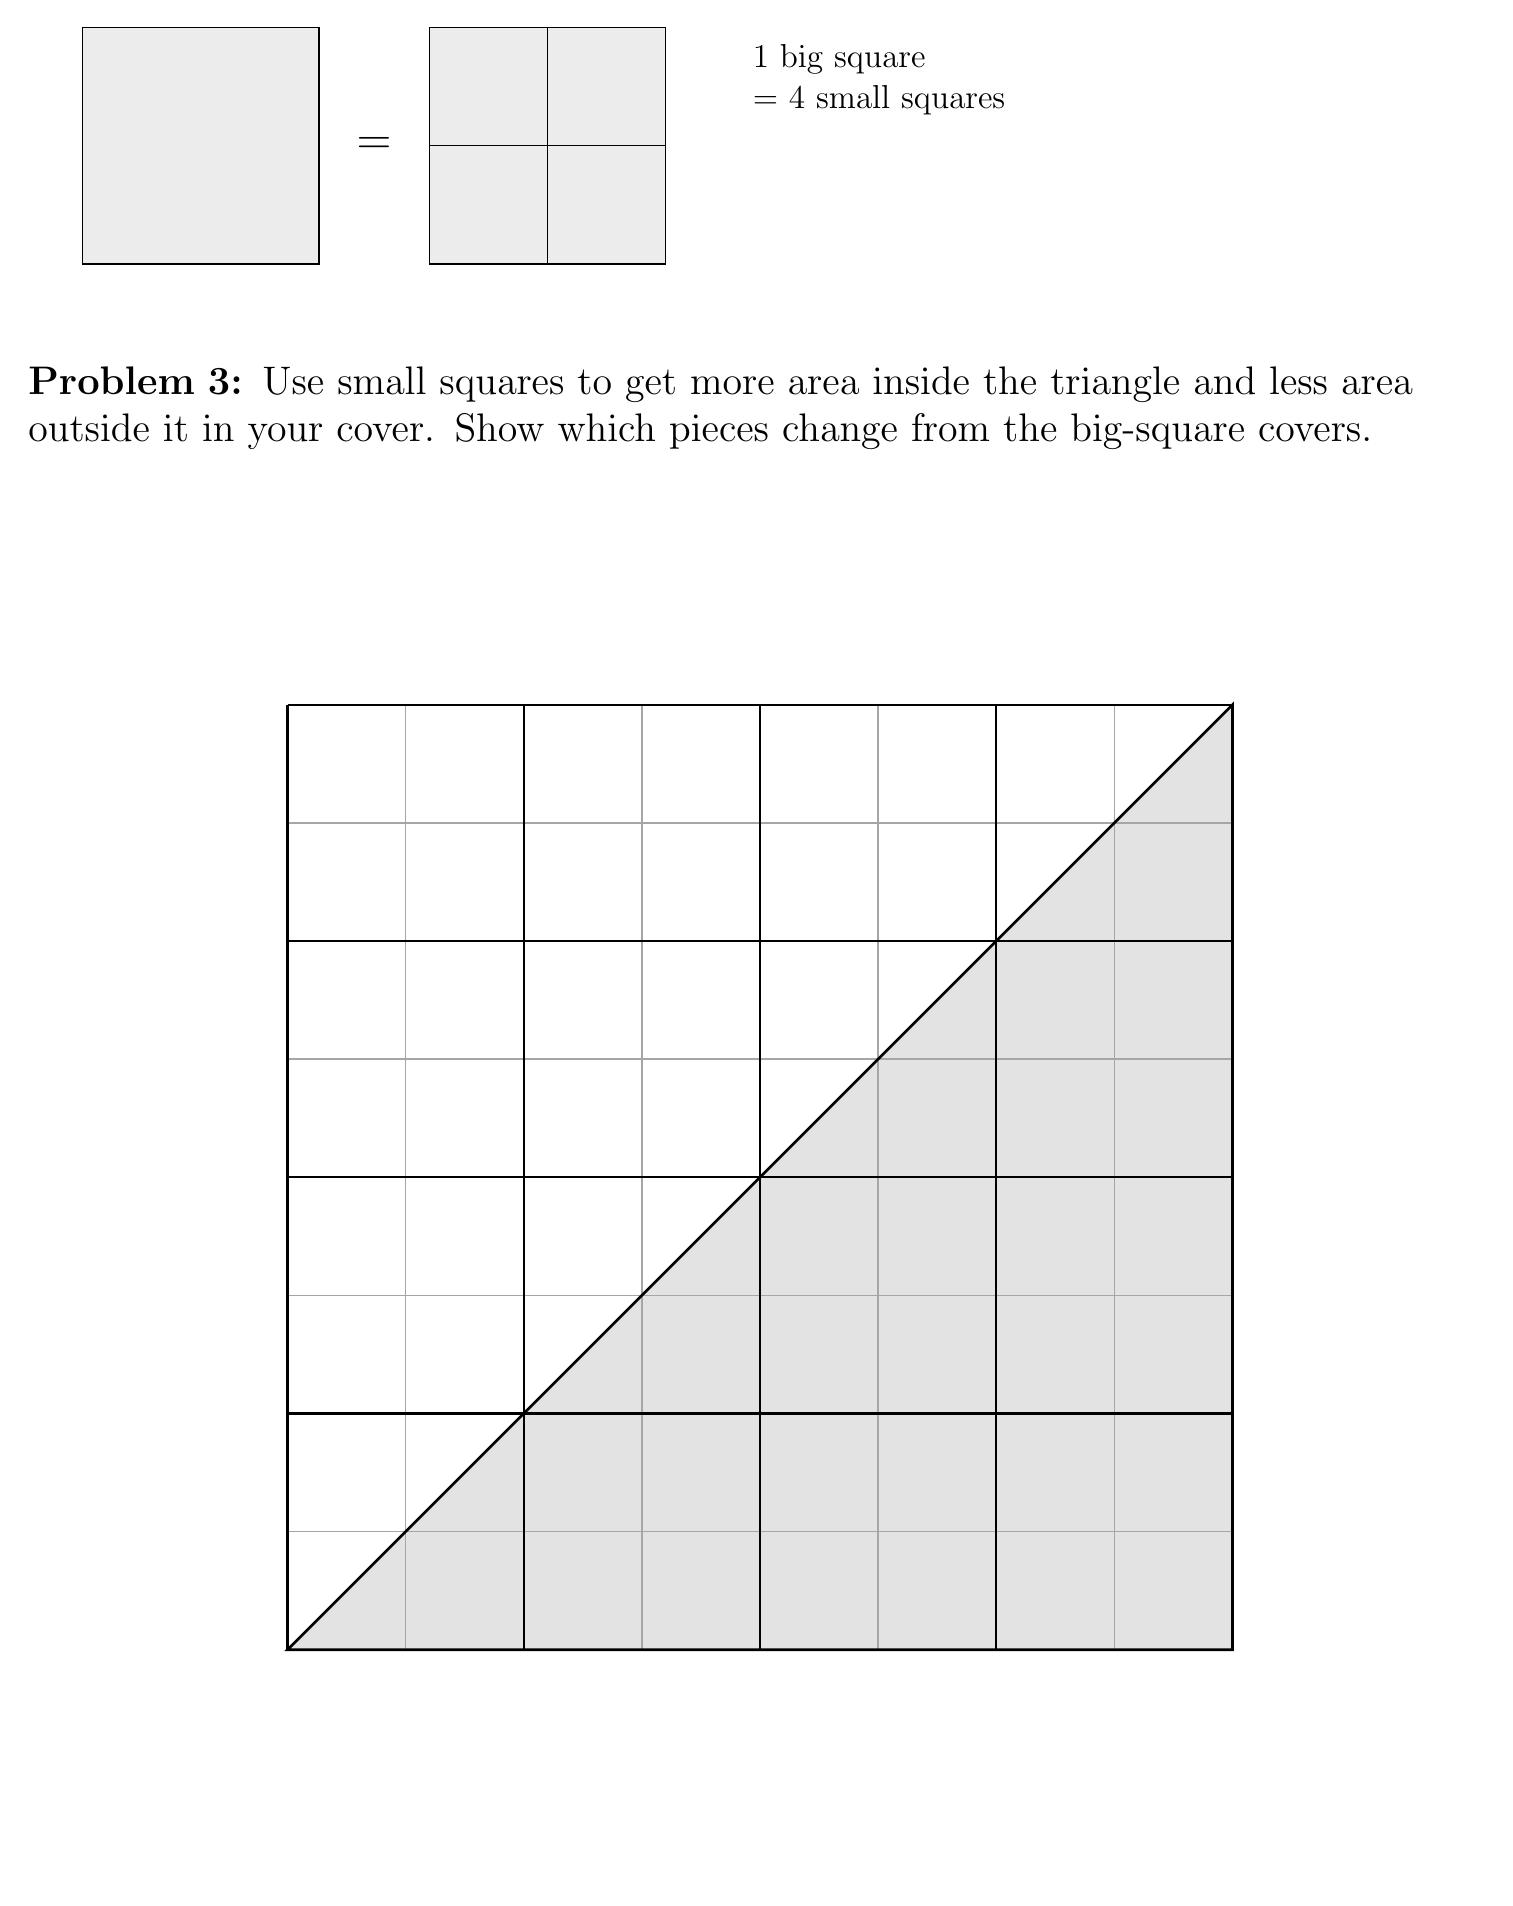
\begin{tikzpicture}[x=1mm,y=-1mm,line width=.5pt]
\path[use as bounding box] (0,0) rectangle (185,235);
\draw[fill=gray!15] (7,0) rectangle ++(30,30);
\node[anchor=center,inner sep=1pt,font=\fontsize{16}{18}\selectfont] at (44,15) {=};
\draw[fill=gray!15] (51,0) rectangle ++(15,15);
\draw[fill=gray!15] (51,15) rectangle ++(15,15);
\draw[fill=gray!15] (66,0) rectangle ++(15,15);
\draw[fill=gray!15] (66,15) rectangle ++(15,15);
\node[anchor=north west,inner sep=0pt,text width=83mm,font=\fontsize{12}{15}\selectfont] at (92,2) {1 big square\\ = 4 small squares};
\node[anchor=north west,inner sep=0pt,text width=180mm,font=\fontsize{14}{17}\selectfont] at (0,43) {\textbf{Problem 3:} Use small squares to get more area inside the triangle and less area outside it in your cover. Show which pieces change from the big-square covers.};
\fill[gray!22] (33.0,206.0) -- (153.0,206.0) -- (153.0,86.0) -- cycle;
\draw[gray!70] (33.0,86) -- (33.0,206);
\draw[gray!70] (33,86.0) -- (153,86.0);
\draw[gray!70] (48.0,86) -- (48.0,206);
\draw[gray!70] (33,101.0) -- (153,101.0);
\draw[gray!70] (63.0,86) -- (63.0,206);
\draw[gray!70] (33,116.0) -- (153,116.0);
\draw[gray!70] (78.0,86) -- (78.0,206);
\draw[gray!70] (33,131.0) -- (153,131.0);
\draw[gray!70] (93.0,86) -- (93.0,206);
\draw[gray!70] (33,146.0) -- (153,146.0);
\draw[gray!70] (108.0,86) -- (108.0,206);
\draw[gray!70] (33,161.0) -- (153,161.0);
\draw[gray!70] (123.0,86) -- (123.0,206);
\draw[gray!70] (33,176.0) -- (153,176.0);
\draw[gray!70] (138.0,86) -- (138.0,206);
\draw[gray!70] (33,191.0) -- (153,191.0);
\draw[gray!70] (153.0,86) -- (153.0,206);
\draw[gray!70] (33,206.0) -- (153,206.0);
\draw[line width=.8pt] (33.0,86) -- (33.0,206);
\draw[line width=.8pt] (33,86.0) -- (153,86.0);
\draw[line width=.8pt] (63.0,86) -- (63.0,206);
\draw[line width=.8pt] (33,116.0) -- (153,116.0);
\draw[line width=.8pt] (93.0,86) -- (93.0,206);
\draw[line width=.8pt] (33,146.0) -- (153,146.0);
\draw[line width=.8pt] (123.0,86) -- (123.0,206);
\draw[line width=.8pt] (33,176.0) -- (153,176.0);
\draw[line width=.8pt] (153.0,86) -- (153.0,206);
\draw[line width=.8pt] (33,206.0) -- (153,206.0);
\draw[line width=1pt] (33.0,206.0) -- (153.0,206.0) -- (153.0,86.0) -- cycle;
\end{tikzpicture}
\newpage
\noindent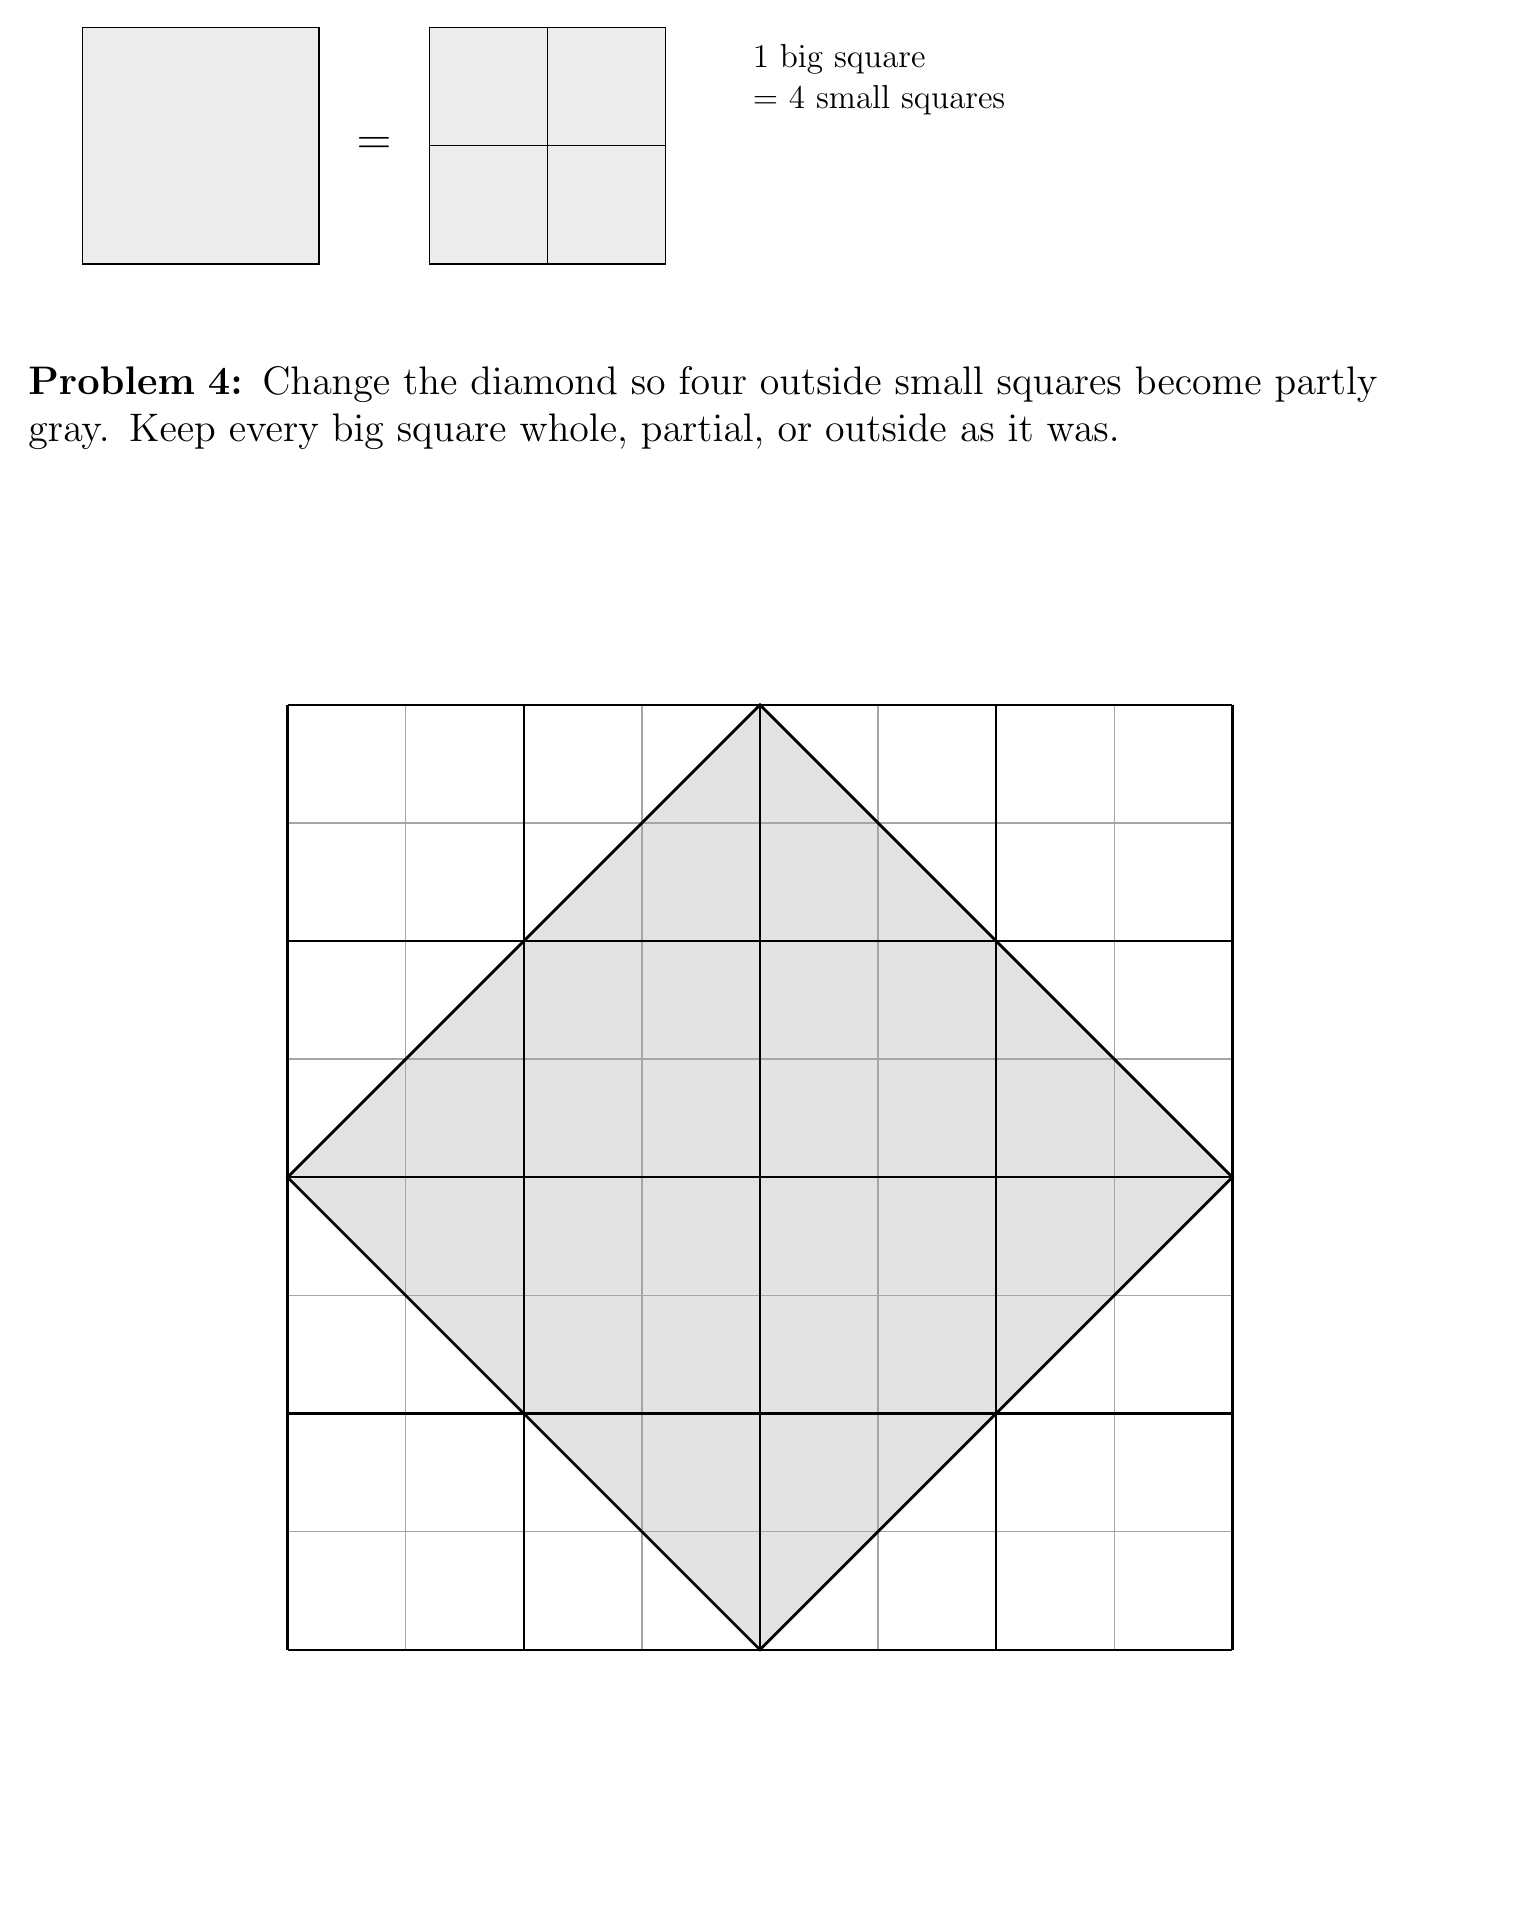
\begin{tikzpicture}[x=1mm,y=-1mm,line width=.5pt]
\path[use as bounding box] (0,0) rectangle (185,235);
\draw[fill=gray!15] (7,0) rectangle ++(30,30);
\node[anchor=center,inner sep=1pt,font=\fontsize{16}{18}\selectfont] at (44,15) {=};
\draw[fill=gray!15] (51,0) rectangle ++(15,15);
\draw[fill=gray!15] (51,15) rectangle ++(15,15);
\draw[fill=gray!15] (66,0) rectangle ++(15,15);
\draw[fill=gray!15] (66,15) rectangle ++(15,15);
\node[anchor=north west,inner sep=0pt,text width=83mm,font=\fontsize{12}{15}\selectfont] at (92,2) {1 big square\\ = 4 small squares};
\node[anchor=north west,inner sep=0pt,text width=180mm,font=\fontsize{14}{17}\selectfont] at (0,43) {\textbf{Problem 4:} Change the diamond so four outside small squares become partly gray. Keep every big square whole, partial, or outside as it was.};
\fill[gray!22] (33.0,146.0) -- (93.0,86.0) -- (153.0,146.0) -- (93.0,206.0) -- cycle;
\draw[gray!70] (33.0,86) -- (33.0,206);
\draw[gray!70] (33,86.0) -- (153,86.0);
\draw[gray!70] (48.0,86) -- (48.0,206);
\draw[gray!70] (33,101.0) -- (153,101.0);
\draw[gray!70] (63.0,86) -- (63.0,206);
\draw[gray!70] (33,116.0) -- (153,116.0);
\draw[gray!70] (78.0,86) -- (78.0,206);
\draw[gray!70] (33,131.0) -- (153,131.0);
\draw[gray!70] (93.0,86) -- (93.0,206);
\draw[gray!70] (33,146.0) -- (153,146.0);
\draw[gray!70] (108.0,86) -- (108.0,206);
\draw[gray!70] (33,161.0) -- (153,161.0);
\draw[gray!70] (123.0,86) -- (123.0,206);
\draw[gray!70] (33,176.0) -- (153,176.0);
\draw[gray!70] (138.0,86) -- (138.0,206);
\draw[gray!70] (33,191.0) -- (153,191.0);
\draw[gray!70] (153.0,86) -- (153.0,206);
\draw[gray!70] (33,206.0) -- (153,206.0);
\draw[line width=.8pt] (33.0,86) -- (33.0,206);
\draw[line width=.8pt] (33,86.0) -- (153,86.0);
\draw[line width=.8pt] (63.0,86) -- (63.0,206);
\draw[line width=.8pt] (33,116.0) -- (153,116.0);
\draw[line width=.8pt] (93.0,86) -- (93.0,206);
\draw[line width=.8pt] (33,146.0) -- (153,146.0);
\draw[line width=.8pt] (123.0,86) -- (123.0,206);
\draw[line width=.8pt] (33,176.0) -- (153,176.0);
\draw[line width=.8pt] (153.0,86) -- (153.0,206);
\draw[line width=.8pt] (33,206.0) -- (153,206.0);
\draw[line width=1pt] (33.0,146.0) -- (93.0,86.0) -- (153.0,146.0) -- (93.0,206.0) -- cycle;
\end{tikzpicture}
\newpage
\noindent\begin{tikzpicture}[x=1mm,y=-1mm,line width=.5pt]
\path[use as bounding box] (0,0) rectangle (185,235);
\node[anchor=north west,inner sep=0pt,text width=180mm,font=\fontsize{14}{17}\selectfont] at (0,0) {\textbf{Problem 5:} Draw two shapes, one at a time, each with 3 whole and 3 partly gray squares. Make one with less than 4 big squares of gray and one with more than 5.};
\draw[gray!70] (33.0,44) -- (33.0,164);
\draw[gray!70] (33,44.0) -- (153,44.0);
\draw[gray!70] (63.0,44) -- (63.0,164);
\draw[gray!70] (33,74.0) -- (153,74.0);
\draw[gray!70] (93.0,44) -- (93.0,164);
\draw[gray!70] (33,104.0) -- (153,104.0);
\draw[gray!70] (123.0,44) -- (123.0,164);
\draw[gray!70] (33,134.0) -- (153,134.0);
\draw[gray!70] (153.0,44) -- (153.0,164);
\draw[gray!70] (33,164.0) -- (153,164.0);
\node[anchor=north west,inner sep=0pt,text width=180mm,font=\fontsize{14}{17}\selectfont] at (0,189) {\textbf{Problem 6:} Keep the same whole and partial squares. Can you make the larger shape bigger again without filling another whole square?};
\node[anchor=north west,inner sep=0pt,text width=180mm,font=\fontsize{12}{15}\selectfont] at (15,223) {One grid square is 1 big-square unit.};
\end{tikzpicture}
\end{document}
